% note: the notes are just thoughts nw had on the highlights of what I had in mind to say when each frame was written. 
% mostly a way for me to get the ball rolling when I hit the frame if I blank
% also has important facts that I just don't want to forget in case it comes up
% they can be enabled/disabled in output as an option to beamer
\documentclass{beamer}
% \setbeameroption{show notes} % comment out to disable notes
% this is only useful if I can present from my PC (likely to not work at all on adobe/ms crap and a gamble on config for other setups):
% \setbeameroption{show notes on second screen=right} 
\usepackage{graphicx}
\mode<presentation>
{
  \usetheme[classification={Distribution Unlimited}]{NRL}
  \logo{
\includegraphics[width=0.1\paperwidth]{NRL_emblem}}
}

\title{Benchmarking GNU Radio on Various General Purpose Processing Architectures}

\author[N\, West \& D.\, Geiger]
{%
  \texorpdfstring{
    \begin{columns}
      \column{.45\linewidth}
      \centering
      Nathan West \\
      \column{.45\linewidth}
      \centering
      Douglas Geiger
    \end{columns}
  }
  {Nathan West \& Douglas Geiger}
}

\institute{U.S. Naval Research Laboratory \\ Mobile Systems Security}


\begin{document}
{
 \section*{Title}
 \begin{frame}
   \titlepage
   {\centering \scriptsize Distribution Statement A: Approved for public release, distribution is unlimited}
 \end{frame}
}

\section*{Outline}
\begin{frame}
  \frametitle{Outline}
  \begin{itemize}
    \item A Brief History
    \item Methodology
    \item Results
    \item Future Work
  \end{itemize}
\end{frame}
\note{\begin{itemize}
  \item Going to cover some previous benchmarks related to GNU Radio
  \item How I went about it
  \item Throw a bunch of graphs at you
  \item Stuff that still needs to be done
\end{itemize}}

\section*{History}
\begin{frame}
  \frametitle{A Brief History of GNU Radio Benchmarks}
  \begin{itemize}
    \item MP-sched, 2008, Eric Blossom 
    \item Architecture Latency Measurements, 2009, George Nychis 
    \item VOLK, 2012, Tom Rondeau 
  \end{itemize}
\end{frame}
\note{\begin{itemize}
\item mp-sched introduced and benchmarked by Eric Blossom in 2008 to test the new multi-processor scheduler. 
He tested performance on a handful of processors using sse and altivec where appropriate.
\item George Nychis used modified UHD and kernel to time the USB delay between USRPs and GNU Radio
\item Tom started work on VOLK in 2010 and released initial benchmarks and tools in February 2012.
\item If you pay attention to GNU Radio mailing list about once or twice a month someone asks about latency: what time can I expect this code to run in?
Now we use Eric Blossom's and Tom's tools (slightly modified) to collect data for a bunch of processors.
\end{itemize}}


\section*{Methodology}
\begin{frame}
  \frametitle{Benchmarking GNU Radio}
  We attempt to measure
  \begin{itemize}
    \item Effectiveness of multi-processor
    \item Time through a block
  \end{itemize}
  Other useful measurements (endless list)
  \begin{itemize}
    \item Total system latency
    \item Symbol analysis (oprofile)
    % there's obviously more, I'll add some on Weds night/Thurs when I have some time to think about it/reread the paper
  \end{itemize} 
\end{frame}
\note{\begin{itemize}
  \item In benchmarking anything the first decision is what to measure. 
  Since tools for some measurements are already available, start there. 
  \item Using Eric's MPsched tools to measure effectiveness of the multiple cores in a processor. 
  \item Using Tom's volk scripts to time billions of samples through blocks.
  \item We also use oprofile to get a list of frequently used symbols in an application to guide further optimization.
  \item There's plenty of place for future benchmarks including total system latency: how long from moment em-wave hits antenna to the response out of DAC?
\end{itemize}}


\begin{frame}
\note{\begin{itemize}
\item In the ideal benchmark the hardware/software under test is the only difference. 
\item This isn't exactly possible, but we tried by using open embedded to build the same image for x86\_64 and ARM procs.
\item This brought some complexities, the final result wound up being the Poky distribution with the meta-oe layer along with masks to get rid of systemd packages that broke the boot process. \\
discuss oe more, assume this crowd doesn't know meta-oe or Poky

\item oprofile allows us to look at applications we care about to see a symbol breakdown of what uses the most processor time.
\end{itemize}}
  \frametitle{Supporting Software}
  \begin{itemize}
    \item Open Embedded
    \item oprofile
    % again, there's more but I'm blanking right now-- add more after rereading paper
  \end{itemize}
\end{frame}

\begin{frame}
\note{
Mention somewhere the change in storage format?
}
  \frametitle{Benchmark Process}
  \begin{enumerate}
    \item Wipe out any residual volk profile results
    \item Run 10x10 mp-sched
    \item volk\_math and volk\_types
    \item volk profile (Determine best SIMD architectures)
    \item Repeat 2 and 3
  \end{enumerate}
\end{frame}

\section*{Results}
\begin{frame}
  \frametitle{Benchmarked Processors}
  \begin{itemize}
    \item Intel i7
    \item Intel Atom
    \item AMD E350
    \item ARM Cortex-A8 (Ettus E110)
    \item Quad-core ARM Cortex-A9 (ODROID-X)
    \item zc702 (Zynq board)
  \end{itemize}
\end{frame}
\note{\begin{itemize}
  \item The i7 is "gold-standard" for what I've tested
  \item Intel Atom, dual core low end x86\_64
  \item AMD E350, AMD's competitor to atom
  \item Ettus E110, gumstix board embedded in USRP
%  \item ODROID-X from hardkernel features an ARM Correx A9 in a SoC targeted for tablets
  \item zc702 is a Xilinx chip, ARM Cortex A8 with NEON
\end{itemize}}

\begin{frame}
  \frametitle{FFT MP-sched, Atom generic kernel}
  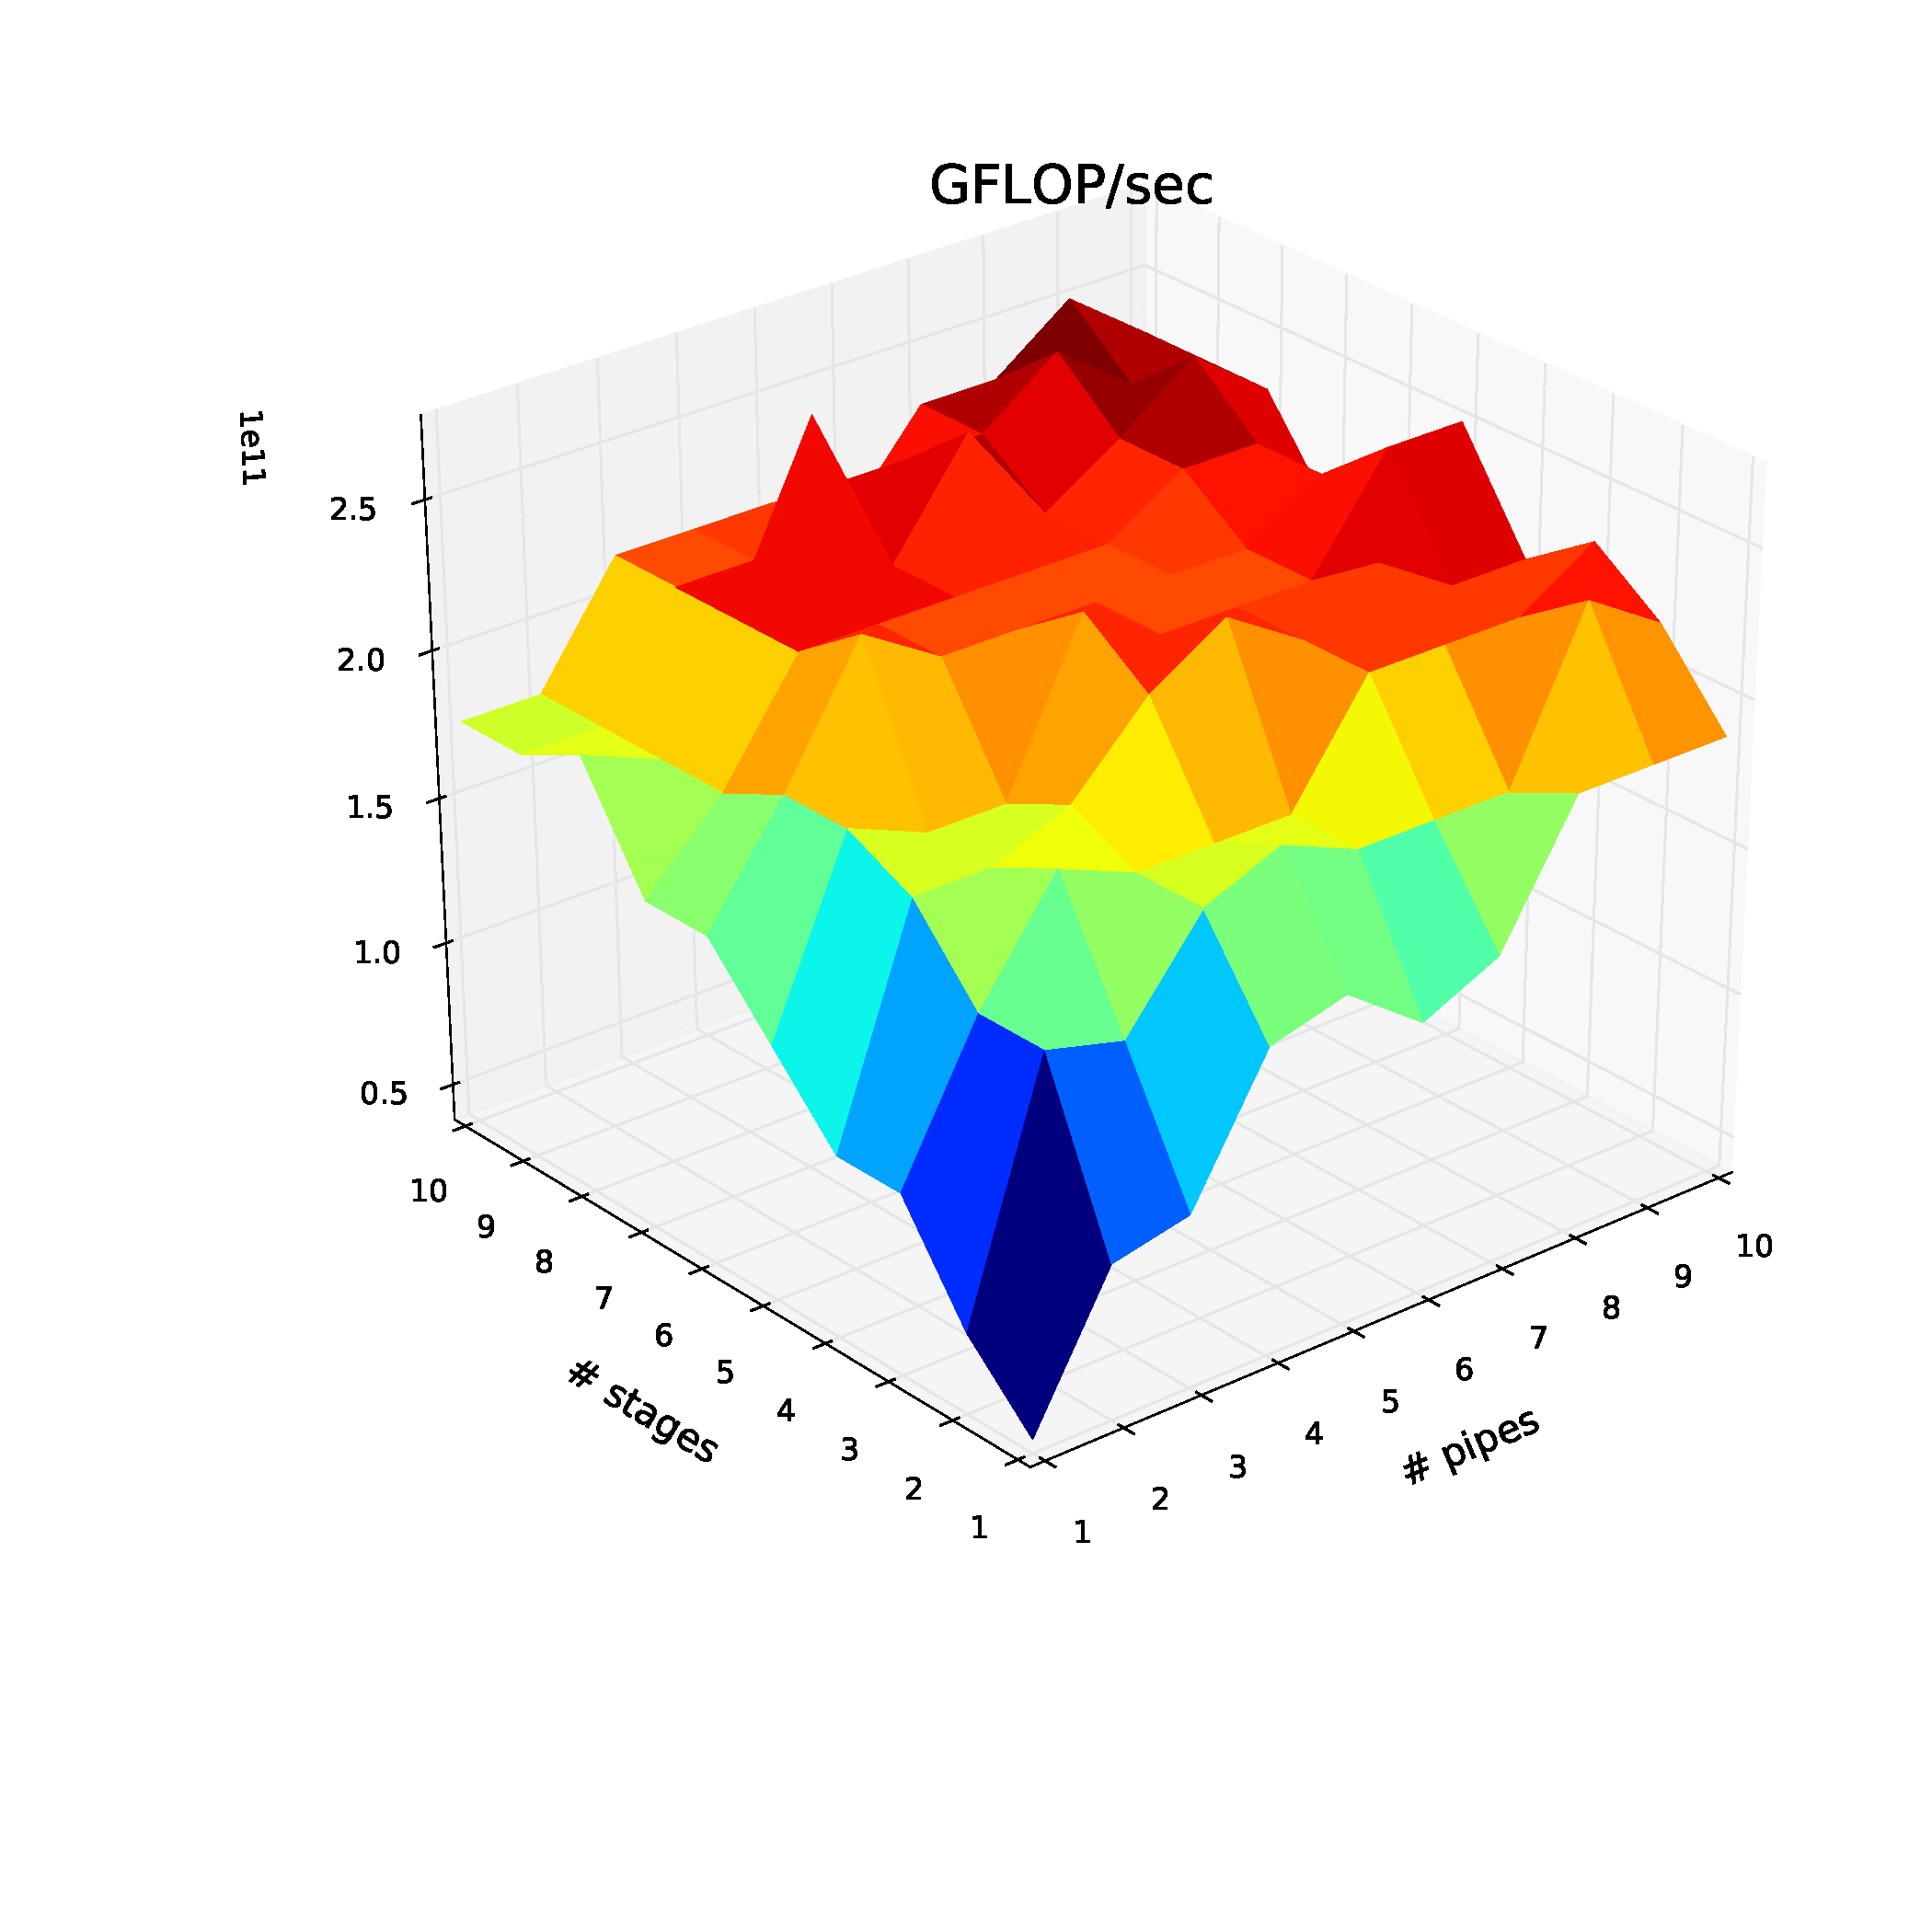
\includegraphics[width=\columnwidth]{../images/fft_i7_generic}
\end{frame}
\begin{frame}
  \frametitle{FFT MP-sched, Atom volked kernel}
  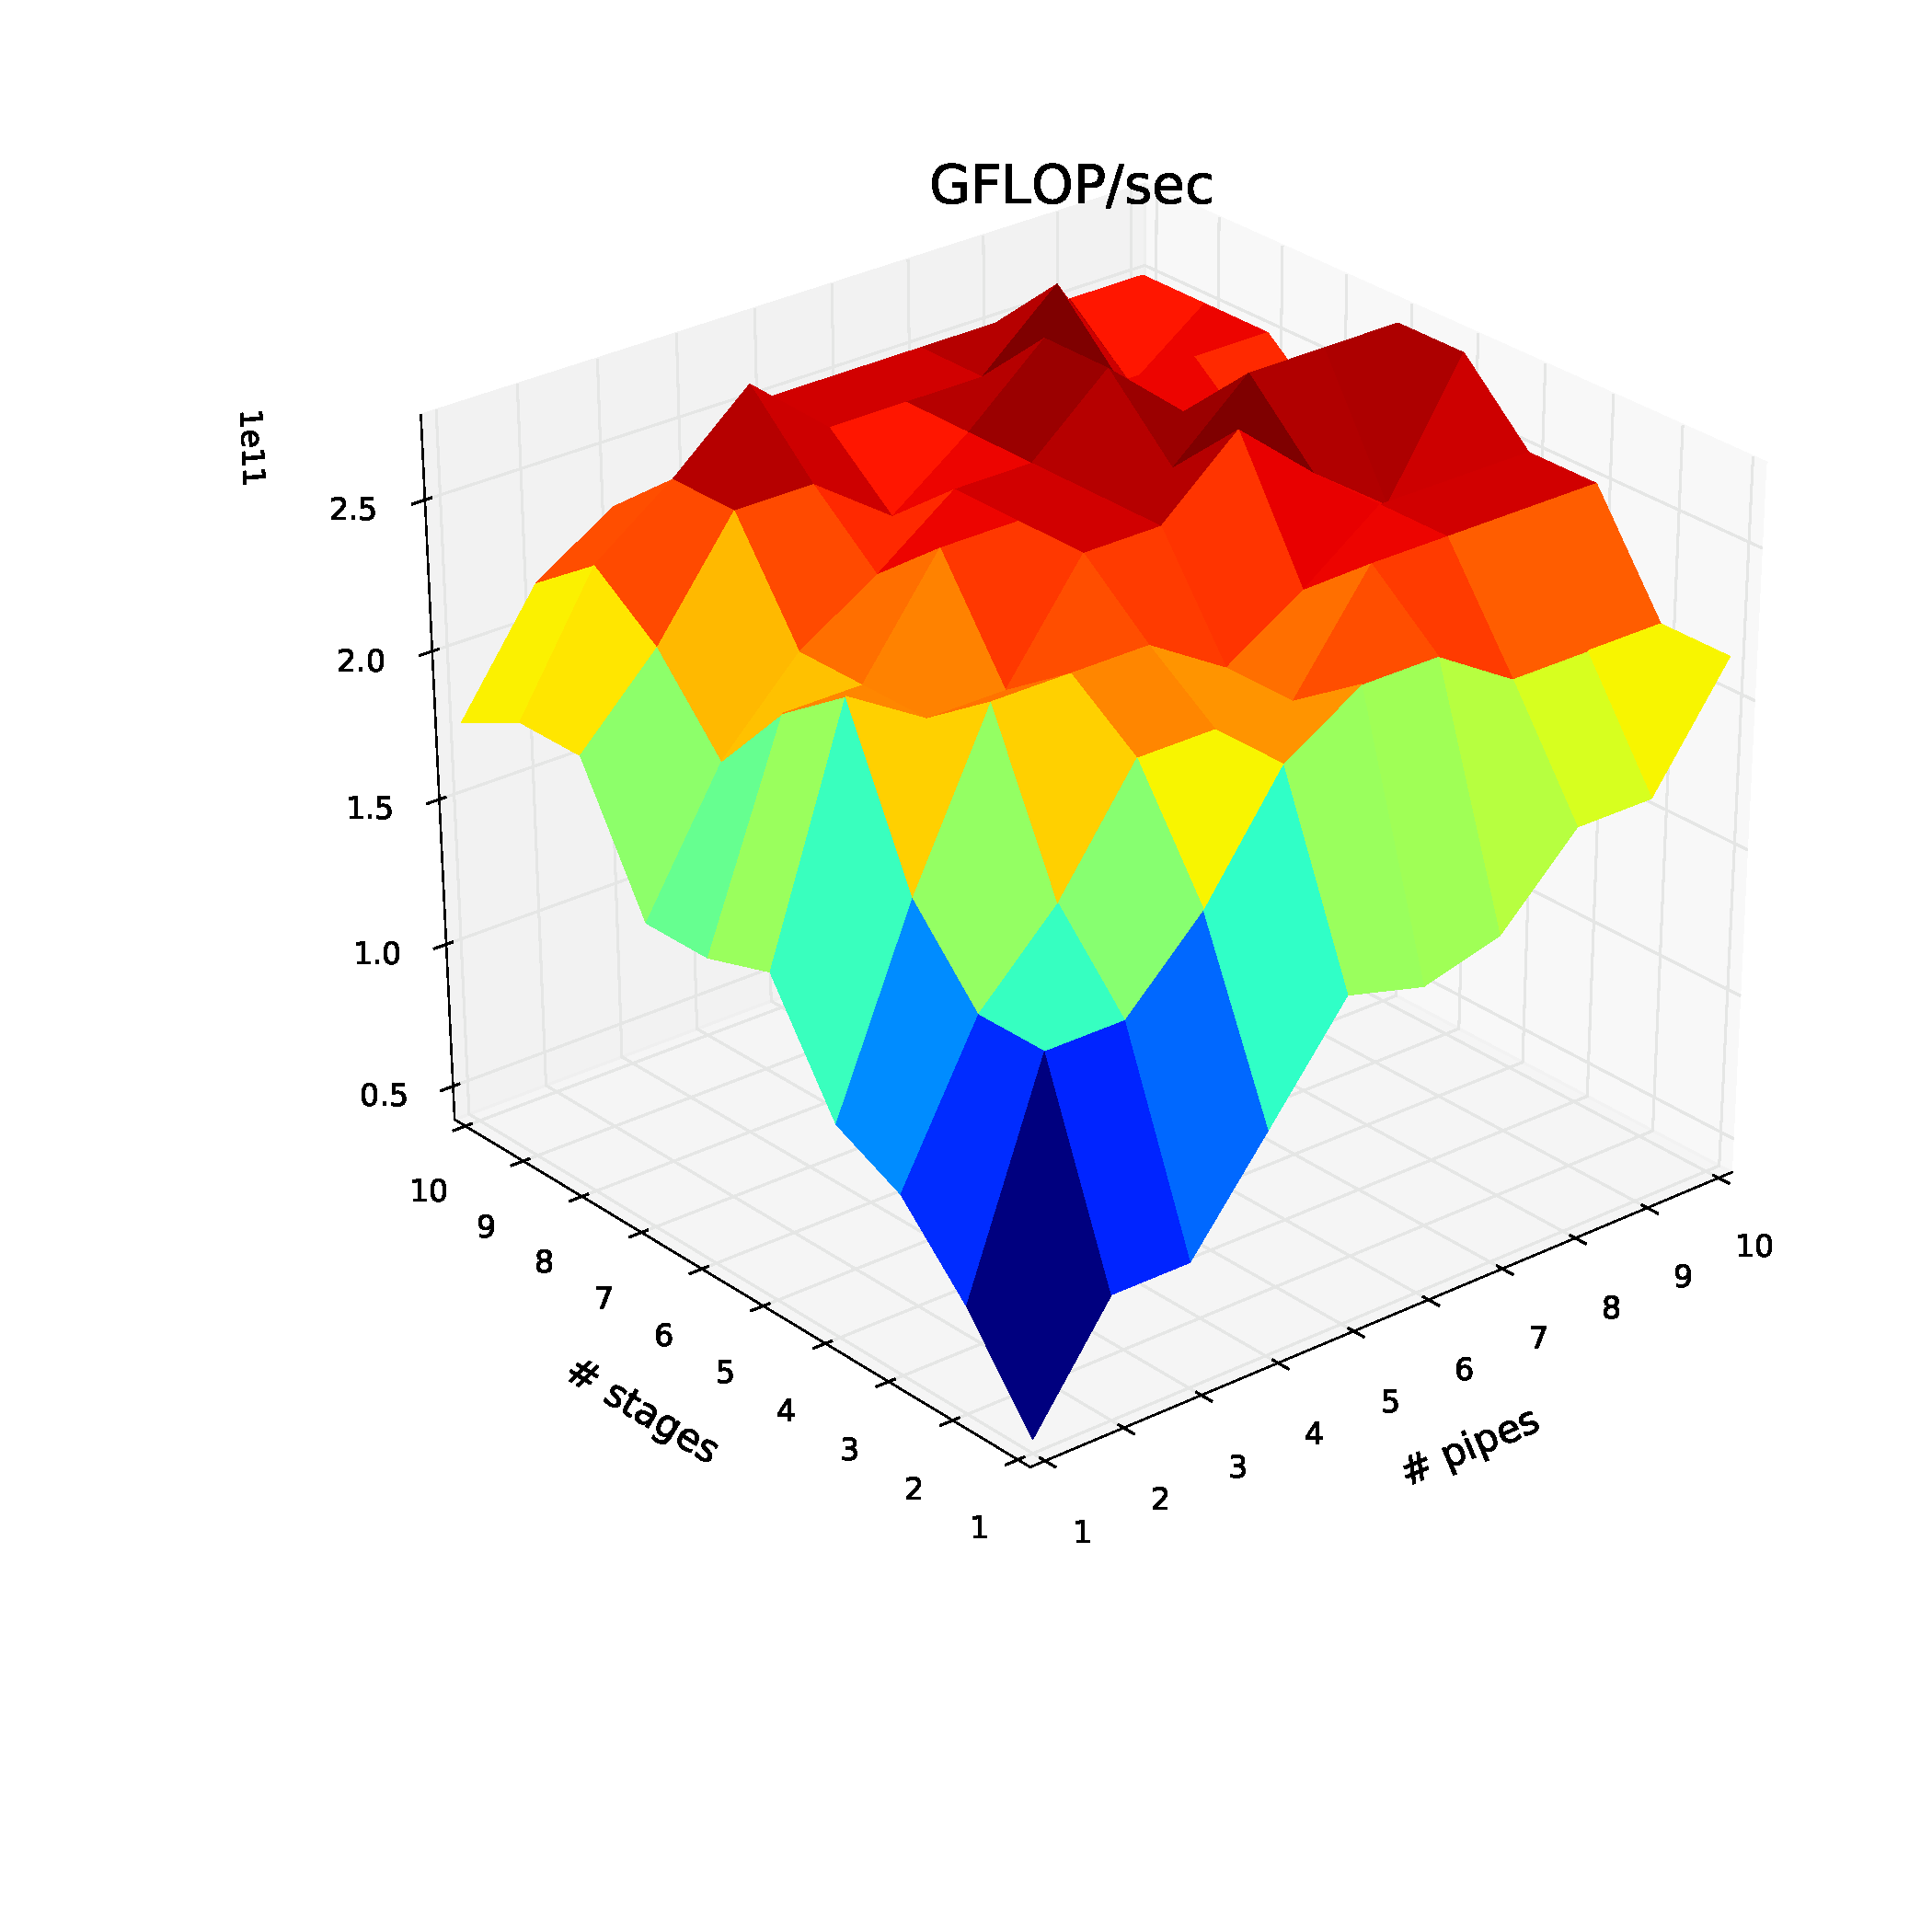
\includegraphics[width=\columnwidth]{../images/fft_i7_volked}
\end{frame}
\begin{frame}
  \frametitle{FIR MP-sched, Atom generic kernel}
  \includegraphics[width=\columnwidth]{../images/fir_i7_generic}
\end{frame}
\begin{frame}
  \frametitle{FIR MP-sched, Atom volked kernel}
  \includegraphics[width=\columnwidth]{../images/fir_i7_volked}
\end{frame}
\begin{frame}
  \frametitle{VOLK Math: all processors generic kernels}
  \includegraphics[width=\columnwidth]{../images/math_generic_compare}
\end{frame}
\begin{frame}
  \frametitle{VOLK Math: all processors volked kernels}
  \includegraphics[width=\columnwidth]{../images/math_volked_compare}
\end{frame}
\begin{frame}
  \frametitle{VOLK Types: all processors generic kernels}
  \includegraphics[width=\columnwidth]{../images/types_generic_compare}
\end{frame}
\begin{frame}
  \frametitle{VOLK Types: all processors volked kernels}
  \includegraphics[width=\columnwidth]{../images/types_volked_compare}
\end{frame}


\begin{frame}
  \frametitle{VOLK Math: all processors (minus i7) generic kernels}
  \includegraphics[width=\columnwidth]{../images/math_generic_compare_noi7}
\end{frame}
\begin{frame}
  \frametitle{VOLK Math: all processors (minus i7) volked kernels}
  \includegraphics[width=\columnwidth]{../images/math_volked_compare_noi7}
\end{frame}
\begin{frame}
  \frametitle{VOLK Types: all processors (minus i7) generic kernels}
  \includegraphics[width=\columnwidth]{../images/types_generic_compare_noi7}
\end{frame}
\begin{frame}
  \frametitle{VOLK Types: all processors (minus i7) volked kernels}
  \includegraphics[width=\columnwidth]{../images/types_volked_compare_noi7}
\end{frame}

\begin{frame}
  \frametitle{VOLK Math: ARM processors generic kernels}
  \includegraphics[width=\columnwidth]{../images/math_generic_arm}
\end{frame}
\begin{frame}
  \frametitle{VOLK Math: ARM processors volked kernels}
  \includegraphics[width=\columnwidth]{../images/math_volked_arm}
\end{frame}
\begin{frame}
  \frametitle{VOLK Types: ARM processors generic kernels}
  \includegraphics[width=\columnwidth]{../images/types_generic_arm}
\end{frame}
\begin{frame}
  \frametitle{VOLK Types: ARM processors volked kernels}
  \includegraphics[width=\columnwidth]{../images/types_volked_arm}
\end{frame}
% all VOLK math/types
% VOLK math/types just ARM procs


\section*{Future Works}
\begin{frame}
  \frametitle{Future Work}
  \begin{itemize}
    \item More hardware!
    \item Add more tests to VOLK suite (modulation)
    \item Latency through graph, and to hardware
  \end{itemize}
\end{frame}

\begin{frame}
  \frametitle{Conclusion}
  \begin{itemize}
    \item Demand for GNU Radio Benchmarks
    \item Using SIMD instructions is important on GPPs
    \item Still a lot to understand
  \end{itemize}
\end{frame}

\end{document}
